\documentclass[11pt,a4paper]{article}

\usepackage[utf8]{inputenc}
\usepackage[T1]{fontenc}
\usepackage[spanish,english]{babel}
\usepackage[a4paper,margin=2.1cm]{geometry}
\usepackage{graphicx}
\usepackage{float}
\usepackage{subcaption}
\usepackage{xcolor}
\usepackage{mdframed}
\usepackage{microtype}
\usepackage{parskip}
\usepackage[colorlinks=true,urlcolor=linkblue,linkcolor=linkblue]{hyperref}

\definecolor{linkblue}{HTML}{14507A}
\definecolor{cajafondo}{HTML}{F2F4F7}
\definecolor{cajaborde}{HTML}{14507A}
\definecolor{notagris}{HTML}{444444}

% El texto que se copia y se pega en el post va en caja. Lo de fuera de la
% caja son notas para Jose y no se publica.
\newmdenv[
  backgroundcolor=cajafondo,
  linecolor=cajaborde,
  linewidth=1.2pt,
  topline=false, bottomline=false, rightline=false,
  innerleftmargin=12pt, innerrightmargin=12pt,
  innertopmargin=10pt, innerbottommargin=10pt,
  skipabove=10pt, skipbelow=10pt
]{post}

\newcommand{\nota}[1]{{\color{notagris}\small #1\par}}
\newcommand{\pie}[1]{\nota{\textbf{Pie de foto sugerido:} #1}}

\title{\vspace{-1.5cm}LINKU camera payload\\[2mm]
       \large Posts para el ISSP, con sus imagenes}
\author{}
\date{26 de noviembre de 2026}

\begin{document}
\selectlanguage{spanish}
\maketitle
\vspace{-1.2cm}

\section*{Como usar esto}

Cinco posts, al largo y al tono del que publico Alvaro sobre el star tracker:
alrededor de 150 palabras, lenguaje llano, una idea por post y un gancho al
siguiente. El texto que va en el post es el que esta \textbf{dentro de la caja
gris}. Todo lo demas son notas y no se publica.

\textbf{Dos cosas que hay que arreglar antes de publicar.} El primero dice
\emph{the second of our three instruments}: cambia el ordinal si el tuyo va
tercero. Y aqui no se nombra la universidad, el estudio ni los socios, asi que
agrega lo que el grupo ya haya acordado decir en publico.

\textbf{Lo que estos posts dejan fuera a proposito}, que es la respuesta si
alguien pregunta por que no hay numeros: ninguna cifra de exactitud, ningun
puntaje de contraste ni de segmentacion, nada de la calibracion, ni el largo
del tether, ni la separacion entre satelites, ni numeros de parte, precios,
proveedores ni fechas. Queda el problema, el enfoque y las partes, que es
exactamente lo que el post de Alvaro da del suyo. \textbf{La unica excepcion
es la figura del post 1}, que es del entregable D5 y trae la base de 100 mm y
el campo de vision escritos: si no los quieres dar, dilo y recorto esa caja.

\textbf{De donde salen las imagenes.} Tres fuentes, todas propias: las
figuras de los entregables, que son las que ya explican el problema con
dibujos hechos para eso; fotos y renders del repositorio; y una captura de
la aplicacion. Ninguna se dibujo para el post.

\vspace{2mm}
\nota{Las arma \texttt{tools/armar\_figuras\_posts.py}, que no inventa
ninguna: recorta, escala y superpone material que ya existe. La captura de la
interfaz la saca \texttt{tools/foto\_gui\_posts.py}, que levanta la ventana
sin camaras. Si cambia alguna, se corren los dos y se vuelve a compilar con
\texttt{.\textbackslash compilar.ps1 "Documentation\textbackslash Posts\_ISSP"}.}

\clearpage
\section*{Post 1. Que es el instrumento}

\begin{post}
\selectlanguage{english}
Hi everyone! Here is the second of our three instruments: the stereo camera
payload.

Its job is to measure a cable. Two satellites fly joined by a thin tether, and
somebody has to know what that tether is actually doing up there: how long it
is, whether it is straight or sagging, how far it reaches away from us. Our
instrument answers that with two cameras and no contact, which is the only way
to measure something you cannot touch and must not disturb.

The prototype is a Raspberry Pi Compute Module 5 with two 12 MP camera
modules, an 8 mm lens on each, and a machined support that holds both cameras
and the computer as one rigid piece. Rigid matters more than it sounds: the
whole measurement comes from the small difference between the two images, so
if the cameras move with respect to each other, the measurement moves with
them.

Next post: why a cable is the hardest thing you can hand to a stereo camera.
\selectlanguage{spanish}
\end{post}

\begin{figure}[H]
  \centering
  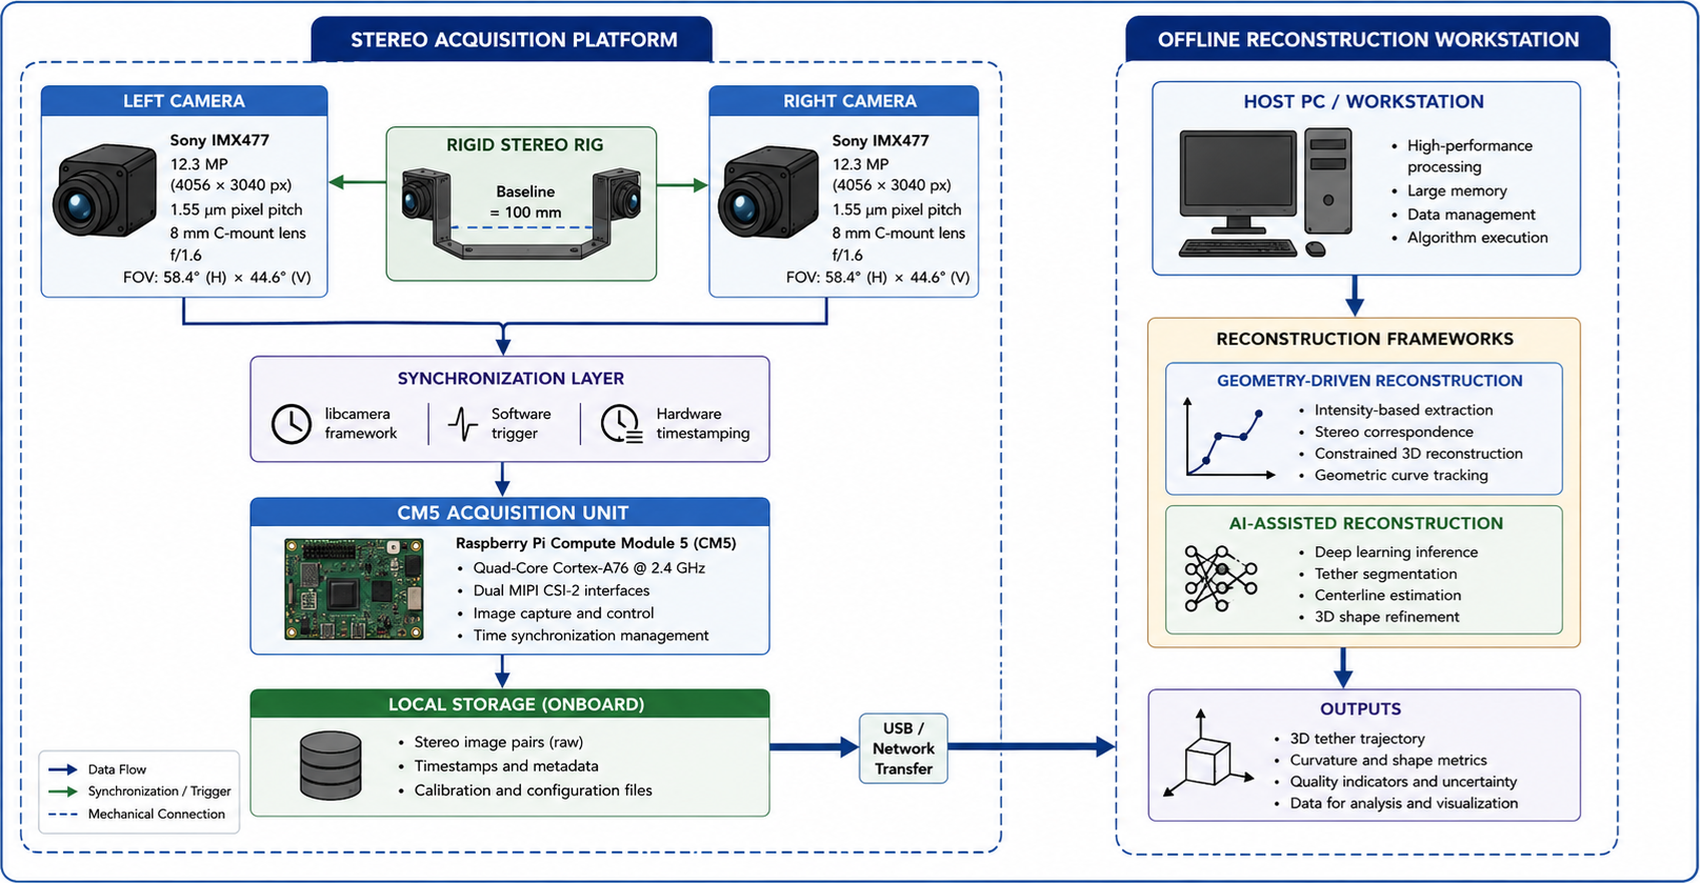
\includegraphics[width=0.98\textwidth]{figures/fig_hw.png}
\end{figure}

\pie{The instrument end to end: two cameras on one rigid rig, a Raspberry Pi
taking and timestamping the pairs, and the reconstruction that happens later
on the ground.}

\nota{Es la \texttt{Figure 5.3} del entregable D5. \textbf{Trae escritos la
base de 100 mm y el campo de vision}, que es lo unico que se sale de la regla
de no dar numeros: si no los quieres, recorto la caja del centro y la figura
sigue funcionando. Hay tambien un CAD del soporte solo
(\texttt{figures/fig\_rig.png}), que es la imagen que tenias y que es mas
pobre: la dejo en la carpeta por si acaso. \textbf{Una foto real del soporte
armado seria mejor que las dos} y no hay ninguna en el repositorio.}

\clearpage
\section*{Post 2. Por que un cable es dificil}

\begin{post}
\selectlanguage{english}
Stereo vision measures distance the way your eyes do. Find the same point in
both images, see how much it shifted between them, and the shift gives you the
depth. The whole method rests on being able to say \emph{the same point}.

A bare cable will not let you. Slide a few centimetres along it and the image
does not change: same brightness, same width, same everything. The two patches
below come from one photograph of ours, hundreds of pixels apart along the
cable, and nothing in either of them says which part of the cable it came
from. Feature-based methods go looking for exactly that kind of distinctive
patch, find nothing to hold on to, and either fail or quietly return noise.

Distance makes it worse. At the ranges we care about the tether is one or two
pixels wide, so there is no shape left to work with, only a faint line on a
dark background.

Next post: what we do instead of matching points.
\selectlanguage{spanish}
\end{post}

\begin{figure}[H]
  \centering
  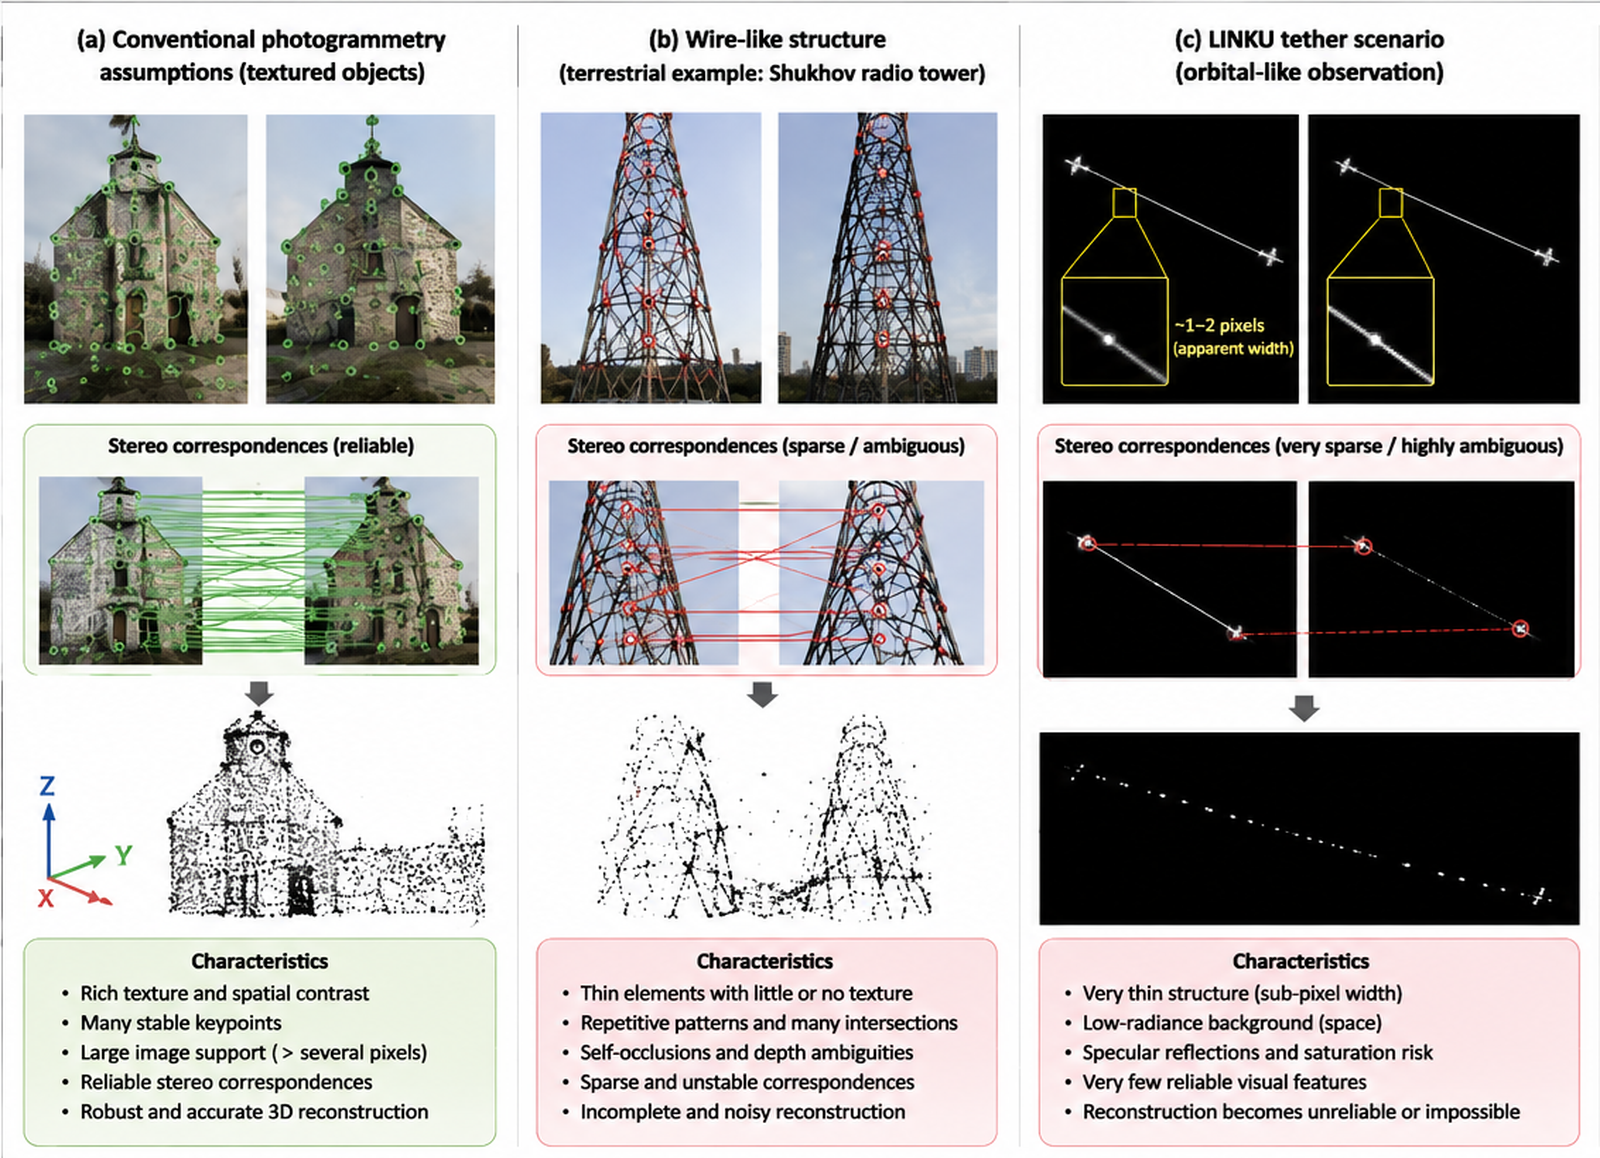
\includegraphics[width=0.66\textwidth]{figures/fig_why.png}
\end{figure}

\vspace{-4mm}
\begin{figure}[H]
  \centering
  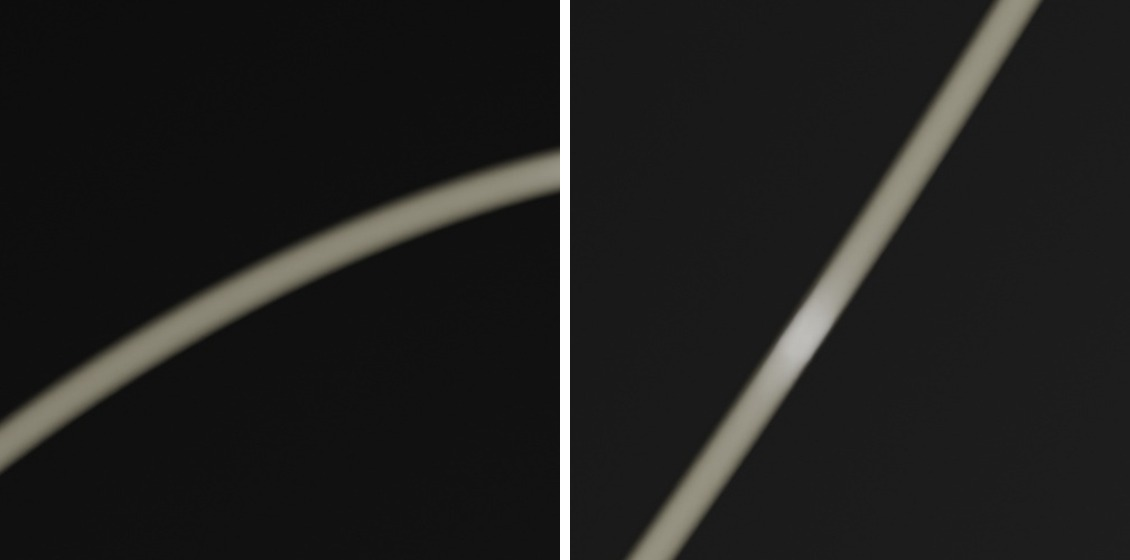
\includegraphics[width=0.46\textwidth]{figures/fig_patches.jpg}
\end{figure}
\vspace{-2mm}

\pie{Top: what a textured building gives a stereo camera (green, every
matched feature), what a steel tower gives it (red, matches that are already
ambiguous), and what a tether gives it. Bottom: two pieces of one of our own
photographs, taken far apart along the same cable.}

\nota{En el post pueden ir como dos imagenes sueltas, que estan en \texttt{figures/}; aqui van pegadas para que la pagina cuadre. Arriba es la \texttt{Figure 2.2} del D5, recortada a sus tres primeras
columnas: la cuarta es un resumen en texto y la leyenda de abajo se queda
fuera, por eso el pie explica el verde y el rojo. Abajo, los dos parches
estan \textbf{separados 1713 px} a lo largo del cable en la misma foto,
elegidos sobre la mascara y descartando los que caen en un cruce. Lo unico
que los distingue es la direccion en la que corre el cable, y esa no dice en
que parte del cable estas.}

\clearpage
\section*{Post 3. Medir una curva, no puntos}

\begin{post}
\selectlanguage{english}
If you cannot match points on a cable, match the cable itself.

Our pipeline treats the tether as one continuous curve instead of a cloud of
features. We separate it from the background in both images, find its two
ends, and trace the path between them, which is the hard part: a hanging
cable crosses in front of itself, and at every crossing the software has to
work out which two branches are the same strand passing through. Then, point
by point along the traced curve, we triangulate. The same place on the cable,
seen from two cameras a known distance apart, gives one position in 3D.

What comes out is not a pretty point cloud. It is a short list of numbers
about the tether: how long it is measured along its own curve, how straight
it is, how far it reaches in depth.

Next post: teaching software to find a cable that is a few pixels wide.
\selectlanguage{spanish}
\end{post}

\begin{figure}[H]
  \centering
  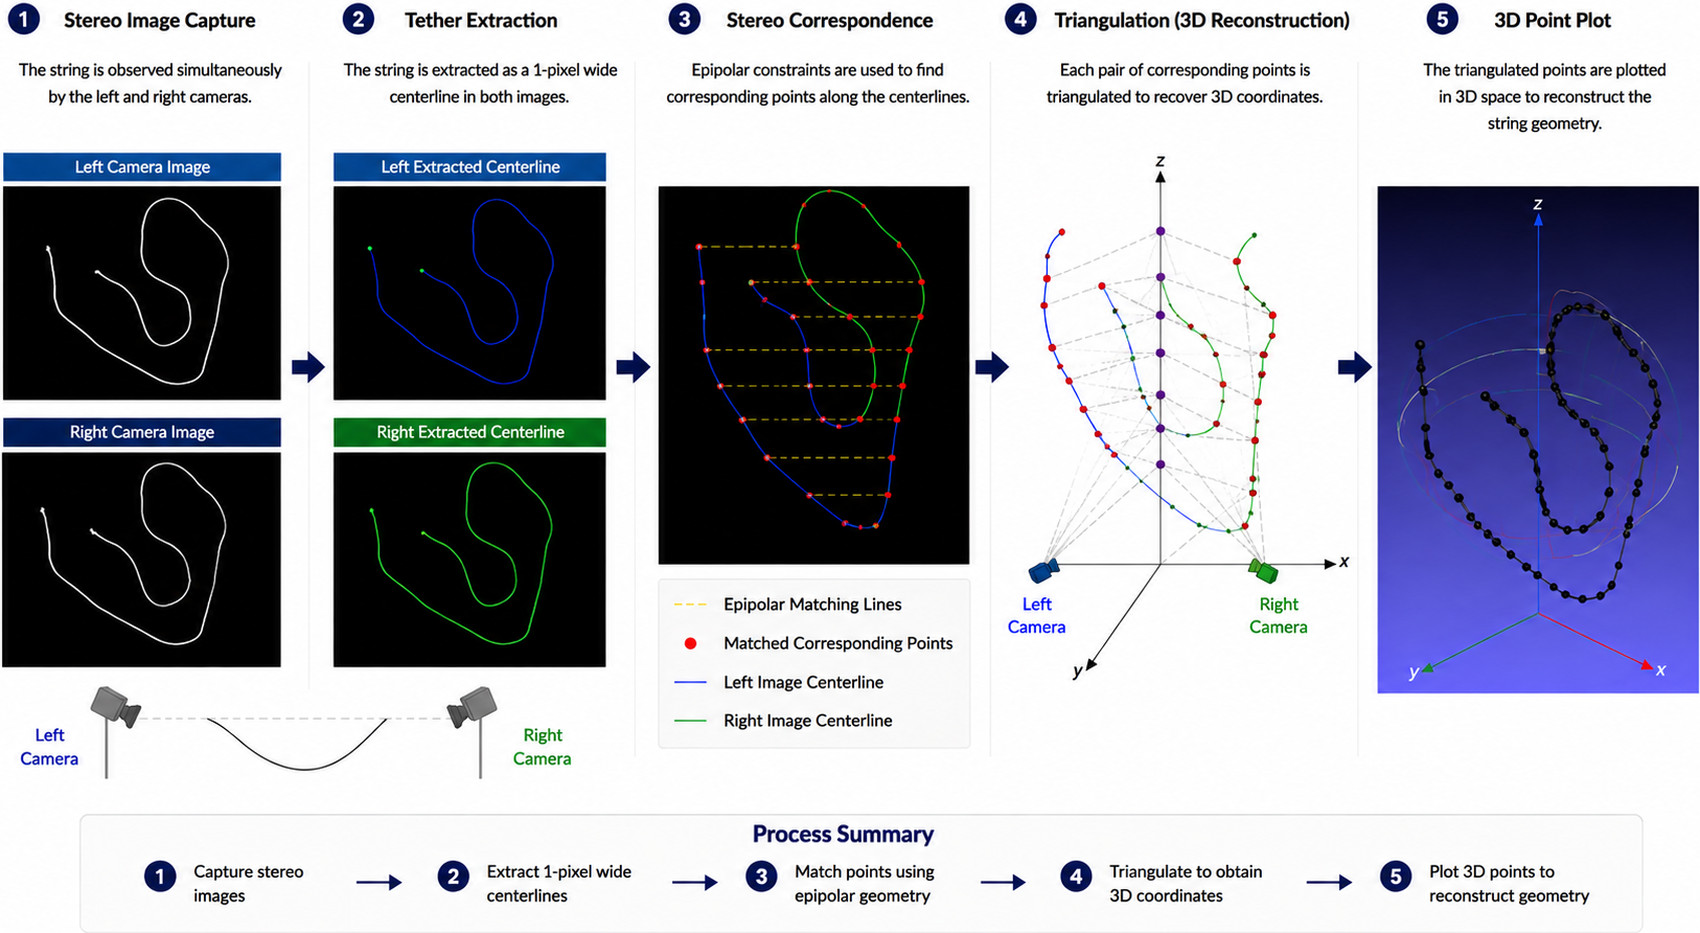
\includegraphics[width=\textwidth]{figures/fig_pipeline.png}
\end{figure}

\pie{The measurement end to end: both cameras see the cable, it is reduced to
a one pixel wide centreline in each image, the two centrelines are paired, and
each pair of points becomes one point in 3D.}

\nota{Es la \texttt{Figure 6.11} del D5. \textbf{Un reparo:} el paso 3 de la
figura dice \emph{epipolar constraints}, y el codigo que corre hoy no empareja
asi, empareja por recorrido, el punto que va al i\% de un trazo con el que va
al i\% del otro. El texto del post no dice epipolar, asi que la figura es lo
unico que lo afirma. Si lo quieres exacto, se puede tapar esa linea de texto o
usar la figura sin el panel 3.}

\clearpage
\section*{Post 4. Encontrar el cable}

\begin{post}
\selectlanguage{english}
Before anything can be measured, the cable has to be separated from
everything else in the frame, and at the distances we work at it is only a few
pixels wide. A hand-tuned threshold does this well in the frame you tuned it
on and badly in the next one.

So we trained a model for it instead. It is not deep learning: it is a
classical machine learning classifier that looks at each pixel through a
handful of descriptors, its colour and how much its neighbourhood looks like a
thin ridge, which is the same kind of detector used to find blood vessels in
medical images. It runs on a laptop in seconds and needs no GPU.

The interesting part was the training data. Hand-labelled frames of a real
cable are slow to produce, so we wrote a generator that draws synthetic scenes
with the cable in a known position, and trained on those plus a few real ones.

Next post: how we test any of this on the ground.
\selectlanguage{spanish}
\end{post}

\begin{figure}[H]
  \centering
  
\includegraphics[width=0.56\textwidth]{figures/fig_mask_overlay.jpg}
\end{figure}

\vspace{-4mm}
\begin{figure}[H]
  \centering
  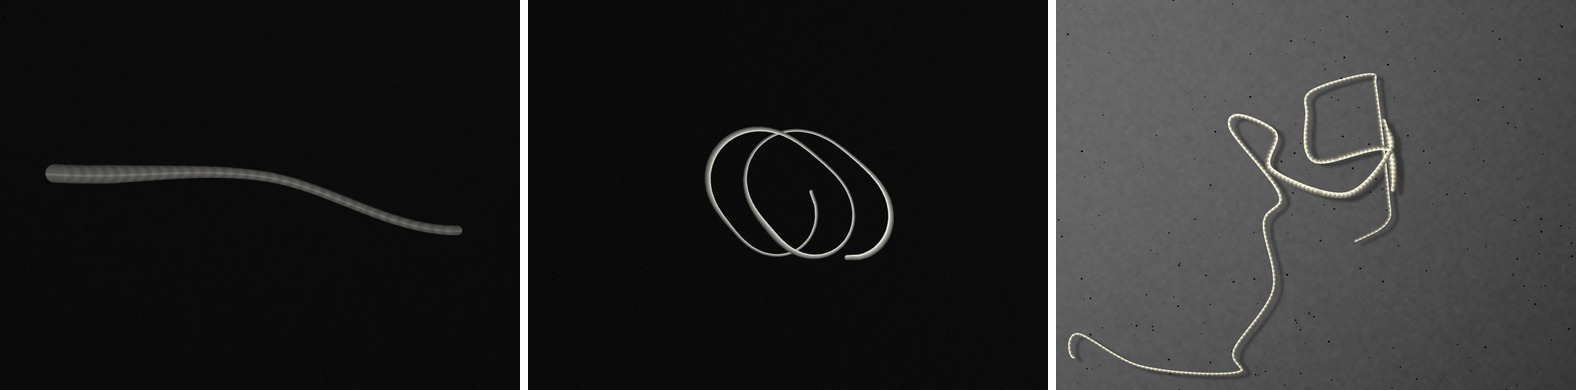
\includegraphics[width=0.93\textwidth]{figures/fig_synthetic_row.jpg}
\end{figure}
\vspace{-2mm}

\pie{Top: one labelled frame, the cable marked in orange and everything else
left out. The dark line crossing it is the cable's own shadow on the wall, and
it is deliberately not marked, because telling the two apart is part of what
the model has to learn. Bottom: three scenes our generator drew by itself, with
the true position of the cable known in each one.}

\nota{Ojo con como se describe la de arriba: esa mascara esta
\textbf{dibujada a mano}, es la etiqueta con la que se entrena, no la salida
del modelo. Por eso el pie dice \emph{labelled frame} y no \emph{found by the
model}. Si prefieres ensenar lo que el modelo produce de verdad, lo corro
sobre un cuadro que no haya visto y cambio la figura. Las tres de abajo salen
de \texttt{data/synthetic}, que no esta versionado: si hace falta rehacer la
figura en otra maquina, primero hay que regenerarlas con \texttt{synthetic/}.}

\clearpage
\section*{Post 5. Probarlo en la oscuridad}

\begin{post}
\selectlanguage{english}
In orbit this instrument works in the dark, with the Sun as the only lamp and
in a direction nobody gets to choose. That is hard to argue about from a desk,
so we test it in a blacked out television studio, with the cable strung across
the room and professional film fixtures standing in for the Sun.

One thing we did not expect to spend time on: where to point the lamps. A
spotlight aimed at a thin cable across many metres lights a bright patch and
leaves the rest dark, and the direction it comes from decides whether the
camera sees a lit cable or a silhouette. Rather than find that out on the day,
we rebuilt the studio in a renderer, with the real fixtures and their real
beam angles, and tried the arrangements there first. The simulation lives
inside the same application that processes the real frames, so the pictures
and the numbers sit next to each other.

The session itself is coming. We will report what the instrument measured, and
where the simulation turned out to be wrong.
\selectlanguage{spanish}
\end{post}

\begin{figure}[H]
  \centering
  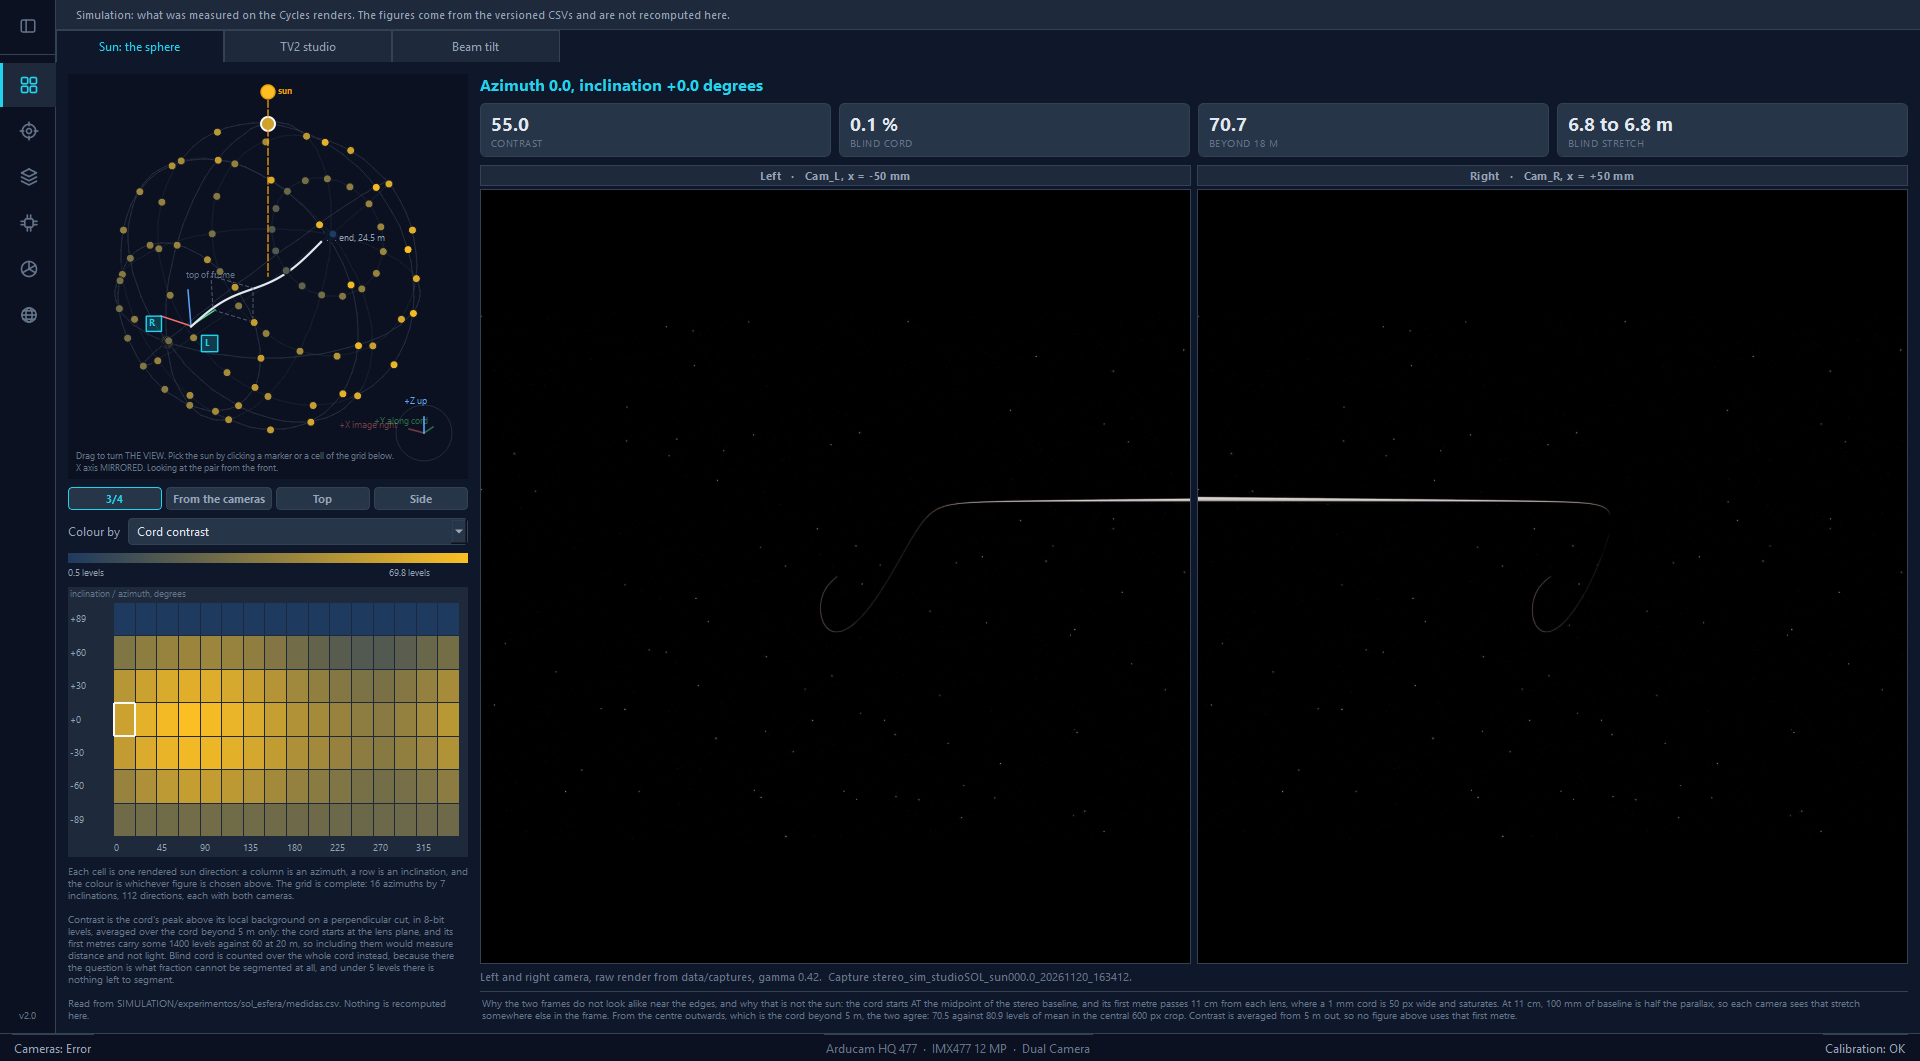
\includegraphics[width=0.78\textwidth]{figures/fig_gui_sphere.png}
\end{figure}

\vspace{-4mm}
\begin{figure}[H]
  \centering
  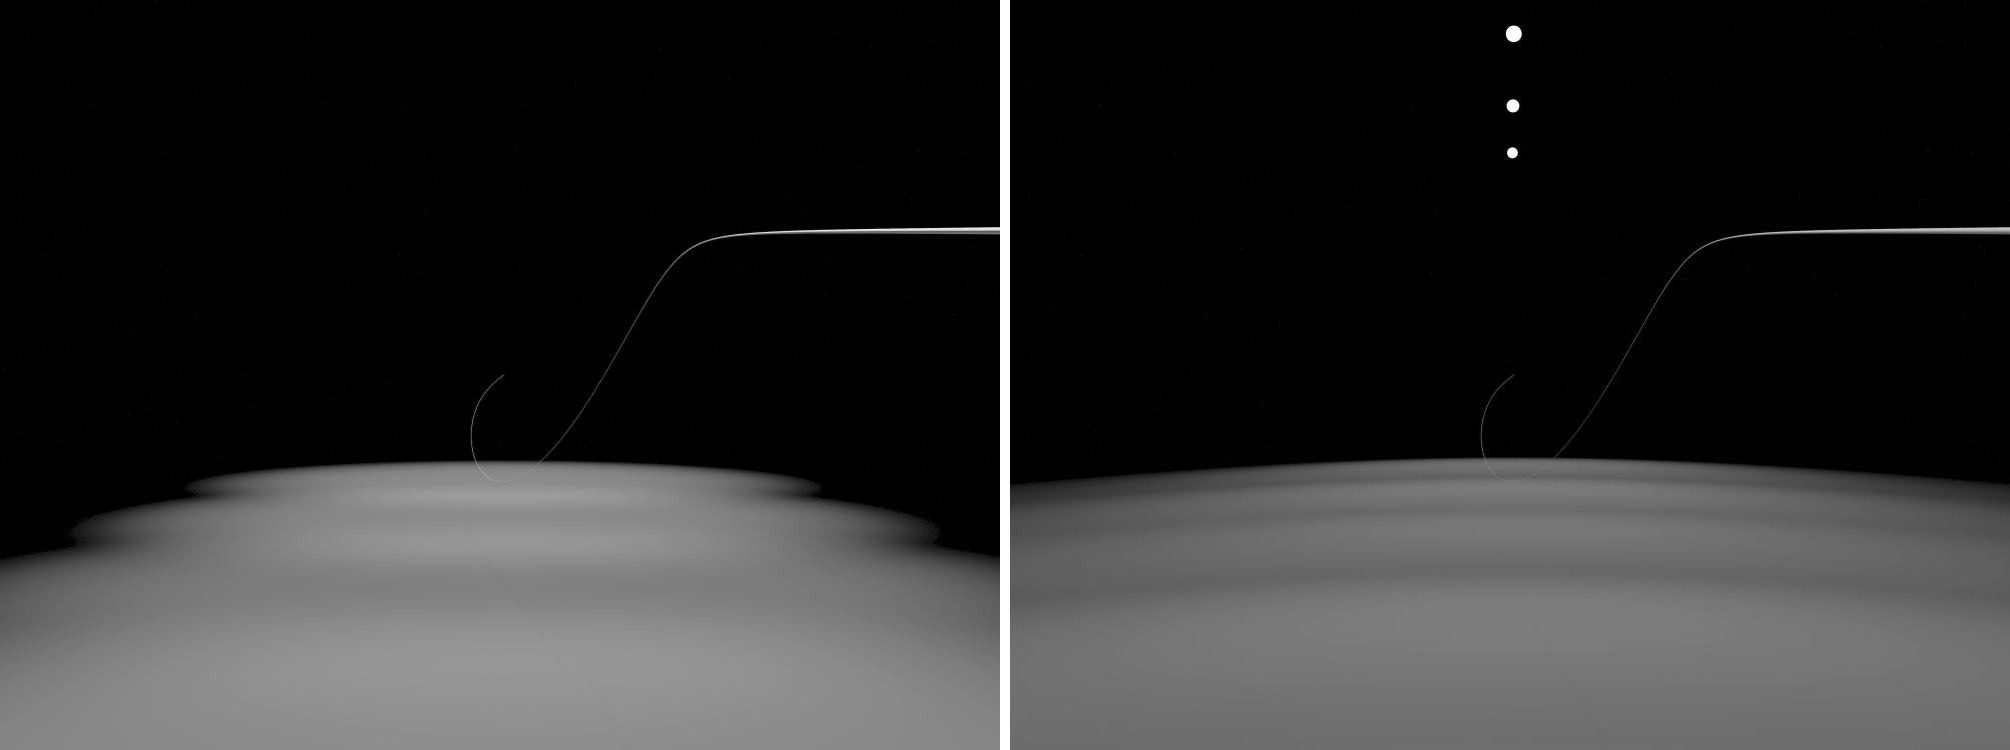
\includegraphics[width=0.84\textwidth]{figures/fig_studio_pair.jpg}
\end{figure}
\vspace{-2mm}

\pie{Top: our own software, with every simulated direction of the Sun on the
left and what the two cameras see from the one you pick on the right. Bottom:
the same room, cable and lamps, with the only difference being where the lamps
are aimed, and on the right they are tilted far enough to come into the shot
themselves.}

\nota{La captura es la pagina Simulation de la aplicacion, pestana de la
esfera. \textbf{Muestra cifras} de contraste y de cordon ciego, que son
resultados de la simulacion y no del instrumento, pero si prefieres no
ensenarlas, recorto la franja de tarjetas y queda el diagrama de la esfera
con el par de camaras, que es lo que se mira igual. Los dos renders de abajo
son camara izquierda, haz vertical y haz inclinado 60 grados; los puntos
blancos son bocas de luminaria dentro del cuadro.}

\clearpage
\section*{Si hace falta un sexto}

Hay uno bueno y seguro sobre calibracion, y no esta escrito todavia: que el
error de reproyeccion no es una medida de calidad, sino el residuo que el
optimizador acaba de minimizar, y que un tablero casi de frente no permite
recuperar la distancia focal por mucho que se repita la toma. La imagen seria
el tablero ChArUco, \texttt{charuco\_board\_5x7.png}, que ya esta en la raiz
del repositorio, o una captura de la pagina de calibracion guiada pidiendo la
pose siguiente. Dilo y lo escribo con el mismo formato.

\end{document}
